\documentclass[11pt,a4paper]{article}
\usepackage{amsmath,amssymb,amsthm}
\usepackage{graphicx}
\usepackage[margin=2.2cm]{geometry}
\usepackage{xcolor}
\usepackage{titlesec}
\usepackage{fancyhdr}
\usepackage{booktabs}
\usepackage{enumitem}
\usepackage{caption}
\usepackage{hyperref}
\hypersetup{colorlinks=true,linkcolor=blue!70!black,urlcolor=blue!70!black}

\definecolor{primary}{RGB}{0,51,102}
\definecolor{accent}{RGB}{204,102,0}

\titleformat{\section}{\Large\bfseries\color{primary}}{\thesection}{1em}{}
\titleformat{\subsection}{\large\bfseries\color{primary!80!black}}{\thesubsection}{1em}{}

\pagestyle{fancy}
\fancyhf{}
\fancyhead[L]{\small\color{primary}Essential Summary}
\fancyhead[R]{\small\color{primary}Li et al.\ (2024)}
\fancyfoot[C]{\thepage}
\renewcommand{\headrulewidth}{0.5pt}

\begin{document}

\begin{center}
{\LARGE\bfseries\color{primary}Essential Summary}\\[12pt]
{\large\bfseries A Modified Generalized Harmonic Function\\Perturbation Method and Its Application\\in Analyzing Generalized Duffing--Harmonic\\--Rayleigh--Li\'enard Oscillator}\\[8pt]
{\normalsize Zhenbo Li, Jin Cai, Linxia Hou}\\[4pt]
{\small\itshape International Journal of Non-Linear Mechanics, Vol.\ 166, 104832 (2024)\\DOI: 10.1016/j.ijnonlinmec.2024.104832}\\[6pt]
{\small\rule{0.7\textwidth}{0.5pt}}\\[4pt]
{\small\color{accent}This is an author-prepared essential summary, not the original paper.\\Please cite the published version.}
\end{center}

\vspace{0.5em}

\section{Background and Motivation}

This is the \textbf{foundational paper} of the MGHFP method series. Many classical analytical methods can analyze nonlinear oscillators quantitatively --- but only when the restoring force and damping are simple. Once the oscillator becomes complicated, these methods \textbf{cannot execute their procedures symbolically} without first assigning numerical values to all system parameters. They can only produce isolated solution snapshots, never a continuous analytical picture of how solutions evolve with changing parameters.

This work introduces the \textbf{modified generalized harmonic function perturbation (MGHFP) method} by embedding the composite Simpson quadrature formula into the classical GHFP framework, enabling the entire perturbation procedure to proceed purely symbolically --- no parameter pre-assignment required. This is the foundation upon which all subsequent MGHFP applications (IJNLM 2025, Phys.\ Scr.\ 2026) are built.

\section{System Model}

The generalized Duffing--Harmonic--Rayleigh--Li\'enard (DHRL) oscillator (Eq.\ 1 from the original paper):

\begin{equation}
\ddot{x} + \frac{\lambda x + \mu x^3}{1 + \nu x^2} = \varepsilon(\mu_c + \mu_2 x^2 + \mu_4 x^4 + \mu_6 x^6 + \mu_{22} \dot{x}^2 + \mu_{24} \dot{x}^4)\dot{x}
\label{eq:model}
\end{equation}
where $\lambda$, $\mu$, $\nu$ are stiffness parameters, and the right side contains a \textbf{6-term generalized nonlinear damping} combining Rayleigh terms ($\dot{x}^2$, $\dot{x}^4$) and Li\'enard terms ($x^2$, $x^4$, $x^6$). The rational restoring force makes this oscillator a maximally challenging test case.

\begin{center}

\includegraphics[width=0.85\textwidth]{p3-fig-p13.png}\\
\captionof{figure}{\textbf{Figure 6.} Potential portrait of the DHRL oscillator. The rich potential landscape enables homoclinic and heteroclinic bifurcations, making this an ideal testbed for the MGHFP method.}
\end{center}

\section{The MGHFP Method}

\subsection{How It Works}

The classical GHFP method proceeds via: (1) nonlinear time transformation $\frac{d\varphi}{dt} = \Phi(\varphi)$, (2) Fourier expansion of the solution $x = a\cos^2\Phi + b$, (3) perturbation expansion $a = a_0 + \varepsilon a_1 + \cdots$, and (4) evaluation of integrals to obtain Fourier coefficients. Step (4) is the bottleneck --- for complicated oscillators, these integrals \textbf{cannot be evaluated analytically}.

\subsection{The MGHFP Fix --- Composite Simpson Integration}

The MGHFP method discretizes the integrals using the composite Simpson quadrature formula:

\begin{equation}
\int_a^b f(x)\,dx \approx \frac{h}{3}\Big[f(x_0) + 4\sum_{i\ \mathrm{odd}} f(x_i) + 2\sum_{i\ \mathrm{even}} f(x_i) + f(x_n)\Big]
\label{eq:simpson}
\end{equation}

By dividing the integration interval into eight equal subintervals, the Fourier coefficients $p_{2i}$ become \textbf{explicit algebraic functions} of $a_0$, $b$, and system parameters. The entire perturbation procedure now runs purely symbolically.

\subsection{Nonlinear Time Transformation Details}

The solution is assumed as $x(t) = a\cos^2\varphi(t) + b$, with the nonlinear time transformation:
\begin{equation}
\frac{d\varphi}{dt} = \Phi(\varphi) = \Phi_0 + \varepsilon\Phi_1 + \cdots
\end{equation}

The zero-order frequency function is:
\begin{equation}
\Phi_0(\varphi) = \frac{\sqrt{2[V(a_0+b) - V(a_0\cos^2\varphi + b)]}}{x'_0(\varphi)}
\end{equation}
where $V(x) = \int g(x)\,dx$ is the potential energy. For complicated $g(x)$, this expression is analytically intractable --- which is precisely why the Simpson discretization is needed. After discretization, $\Phi_0$ is expanded as a Fourier series $\Phi_0(\varphi) = \sum_{i=0}^{M} (p_{2i}\cos 2i\varphi + q_{2i}\sin 2i\varphi)$ with $M=4$.

\section{Key Equations}

\subsection{Amplitude--Parameter Relation (Central Result)}

The analytical relationship between limit cycle amplitude $A$ and control parameter $\mu_c$:

\begin{equation}
\boxed{\mu_c = -\frac{4}{a_0^2(2p_0 - p_4)}\Big(E_2\mu_2 + E_4\mu_4 + E_6\mu_6 + E_{22}\mu_{22} + E_{24}\mu_{24}\Big)}
\label{eq:amplitude}
\end{equation}
where $E_i$ are functions of $a_0$, $b$, and the Fourier coefficients $p_{2i}$ computed via composite Simpson integration. Given system parameters, the limit cycle amplitude is obtained \textbf{analytically} --- no numerical integration needed.

\subsection{Stability Criterion}

\begin{equation}
\boxed{h_0 = \frac{1}{\pi}\int_0^\pi \Big[\mu_c + \sum\mu_i(a_0\cos^2\varphi + b)^i + \sum\mu_{ij}(a_0\cos^2\varphi + b)^i(\dot{x}_0)^2\Big]d\varphi}
\label{eq:stability}
\end{equation}
$h_0 > 0$: unstable; $h_0 = 0$: semi-stable (bifurcation point); $h_0 < 0$: stable.

\subsection{Homoclinic and Heteroclinic Bifurcation Thresholds}

Setting the limit cycle amplitude equal to the saddle point coordinate in Eq.\ \eqref{eq:amplitude} yields the critical $\mu_c^{\mathrm{hom}}$ for homoclinic bifurcation. For heteroclinic bifurcation, the amplitude is set to the coordinates of both connected saddle points, yielding critical $\mu_c^{\mathrm{hetero}}$ values. The variation of $\mu_c^{\mathrm{hetero}}$ with respect to system parameters is analyzed in Figure~8.

\section{Example 1: Limit Cycle Evolution (Section 4.2)}

The following parameters are used: $\lambda=2$, $\mu=1$, $\nu=5$, $\mu_2=-0.88$, $\mu_4=0.39$, $\mu_6=-0.1$, $\mu_{22}=0.17$, $\mu_{24}=0.18$.

\begin{center}
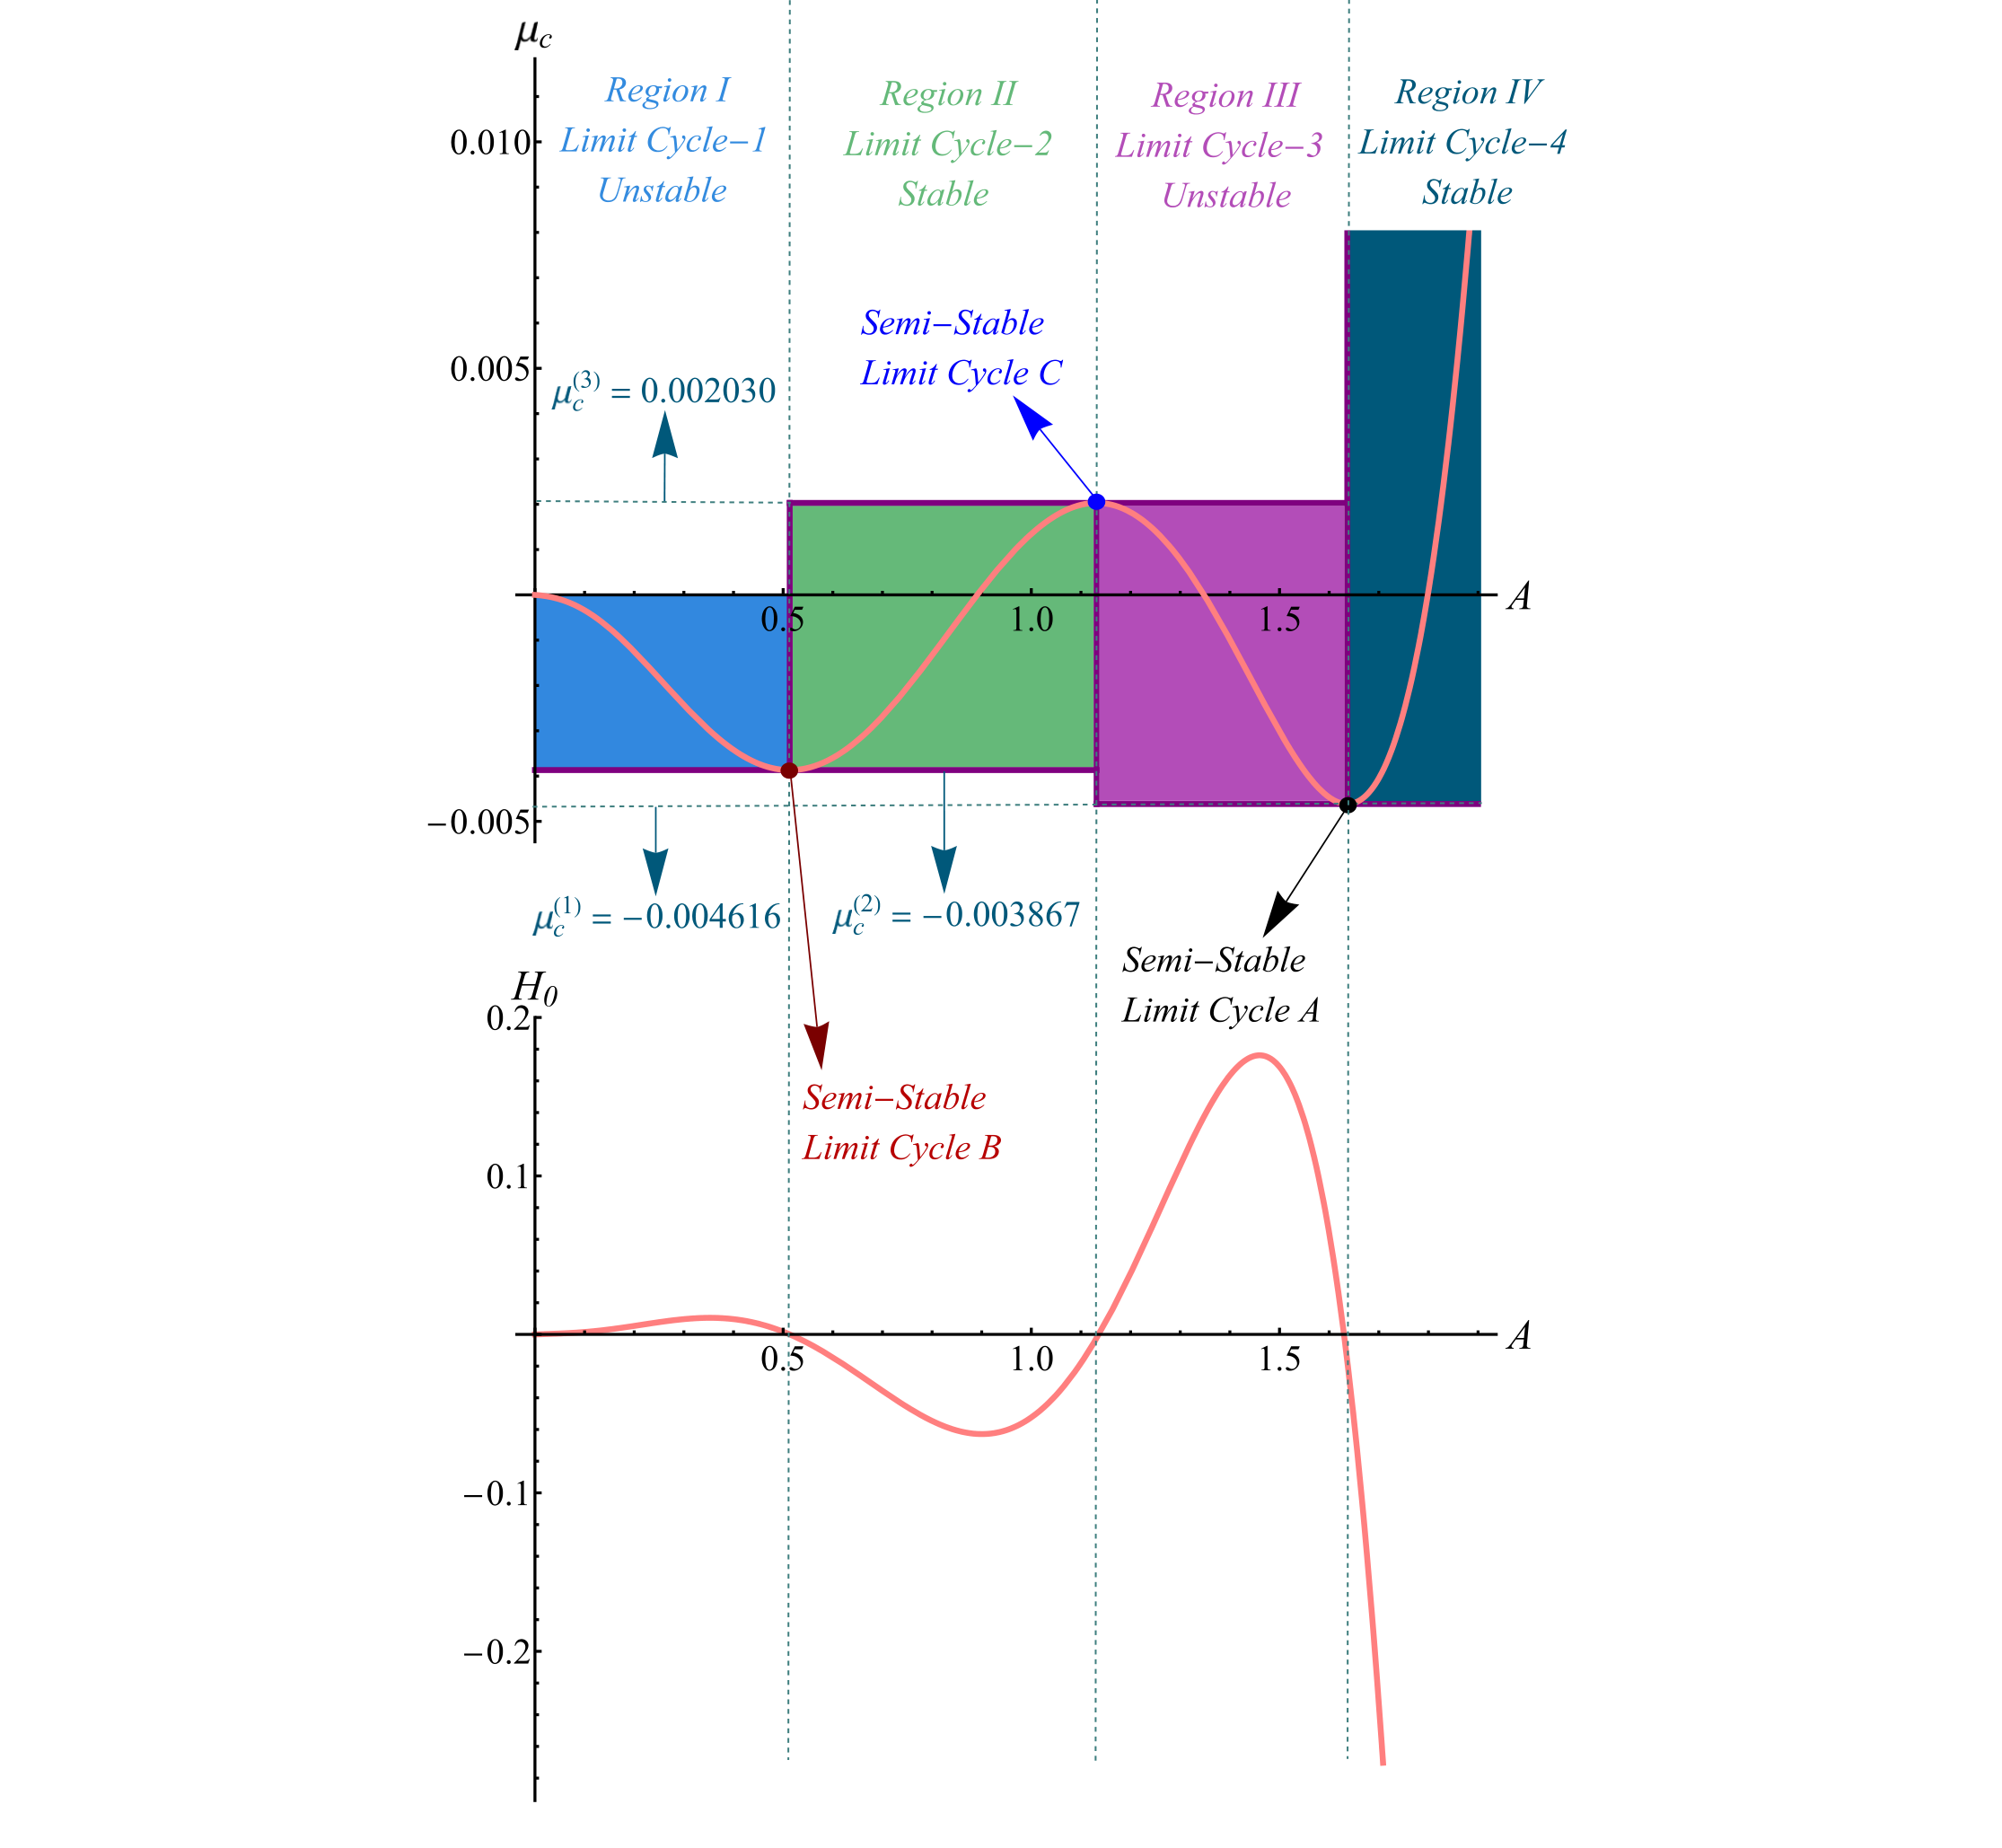
\includegraphics[width=0.75\textwidth]{p3-fig2.png}\\
\captionof{figure}{\textbf{Figure 2.} Evolution of limit cycles in the parametric plane ($\mu_c$--$A$ curve). Four regions (I--IV) identified. Semi-stable bifurcation points A and B mark transitions between regions.}
\label{fig:fig2}
\end{center}

\begin{center}
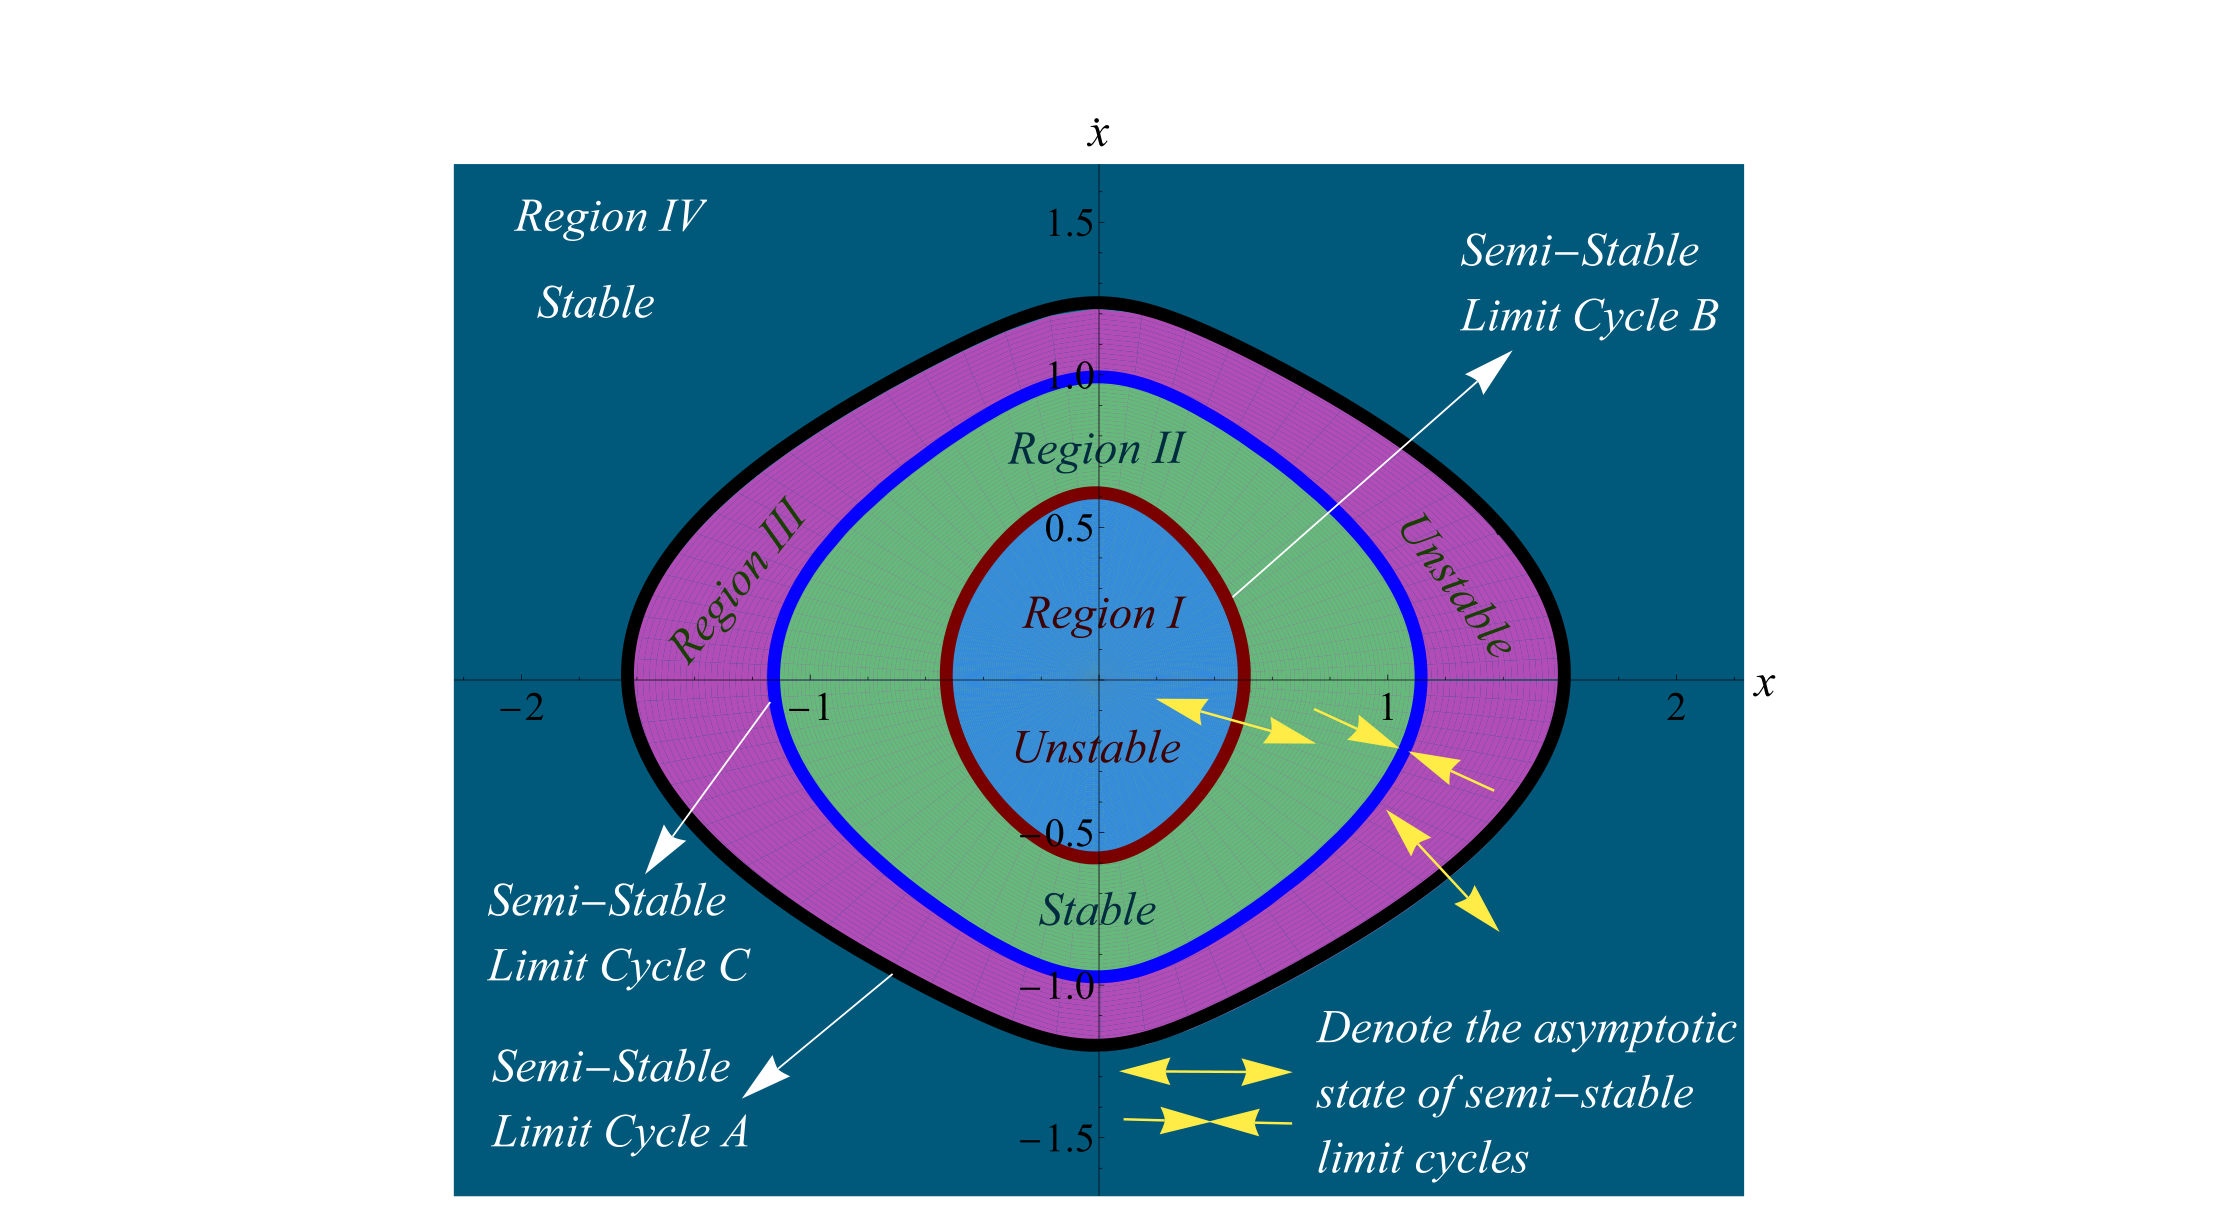
\includegraphics[width=0.85\textwidth]{p3-fig3.png}\\
\captionof{figure}{\textbf{Figure 3.} Phase portraits corresponding to the four regions in Figure~2. The method accurately captures transitions between stability regimes.}
\label{fig:fig3}
\end{center}

Figure~2 reveals the complete limit cycle lifecycle: Region I (no limit cycle), Point A (semi-stable emergence), Region II (stable+unstable coexistence), Point B (second semi-stable bifurcation), Region III (one stable+one unstable), Region IV (single stable cycle persists). Figure~3 provides corresponding phase portraits.

\section{Example 2: Heteroclinic Bifurcation (Section 4.3)}

The heteroclinic bifurcation analysis focuses on deriving \textbf{analytical expressions} for $\mu_c^{\mathrm{hetero}}$, enabling quantitative study of its variation with system parameters.

\begin{center}
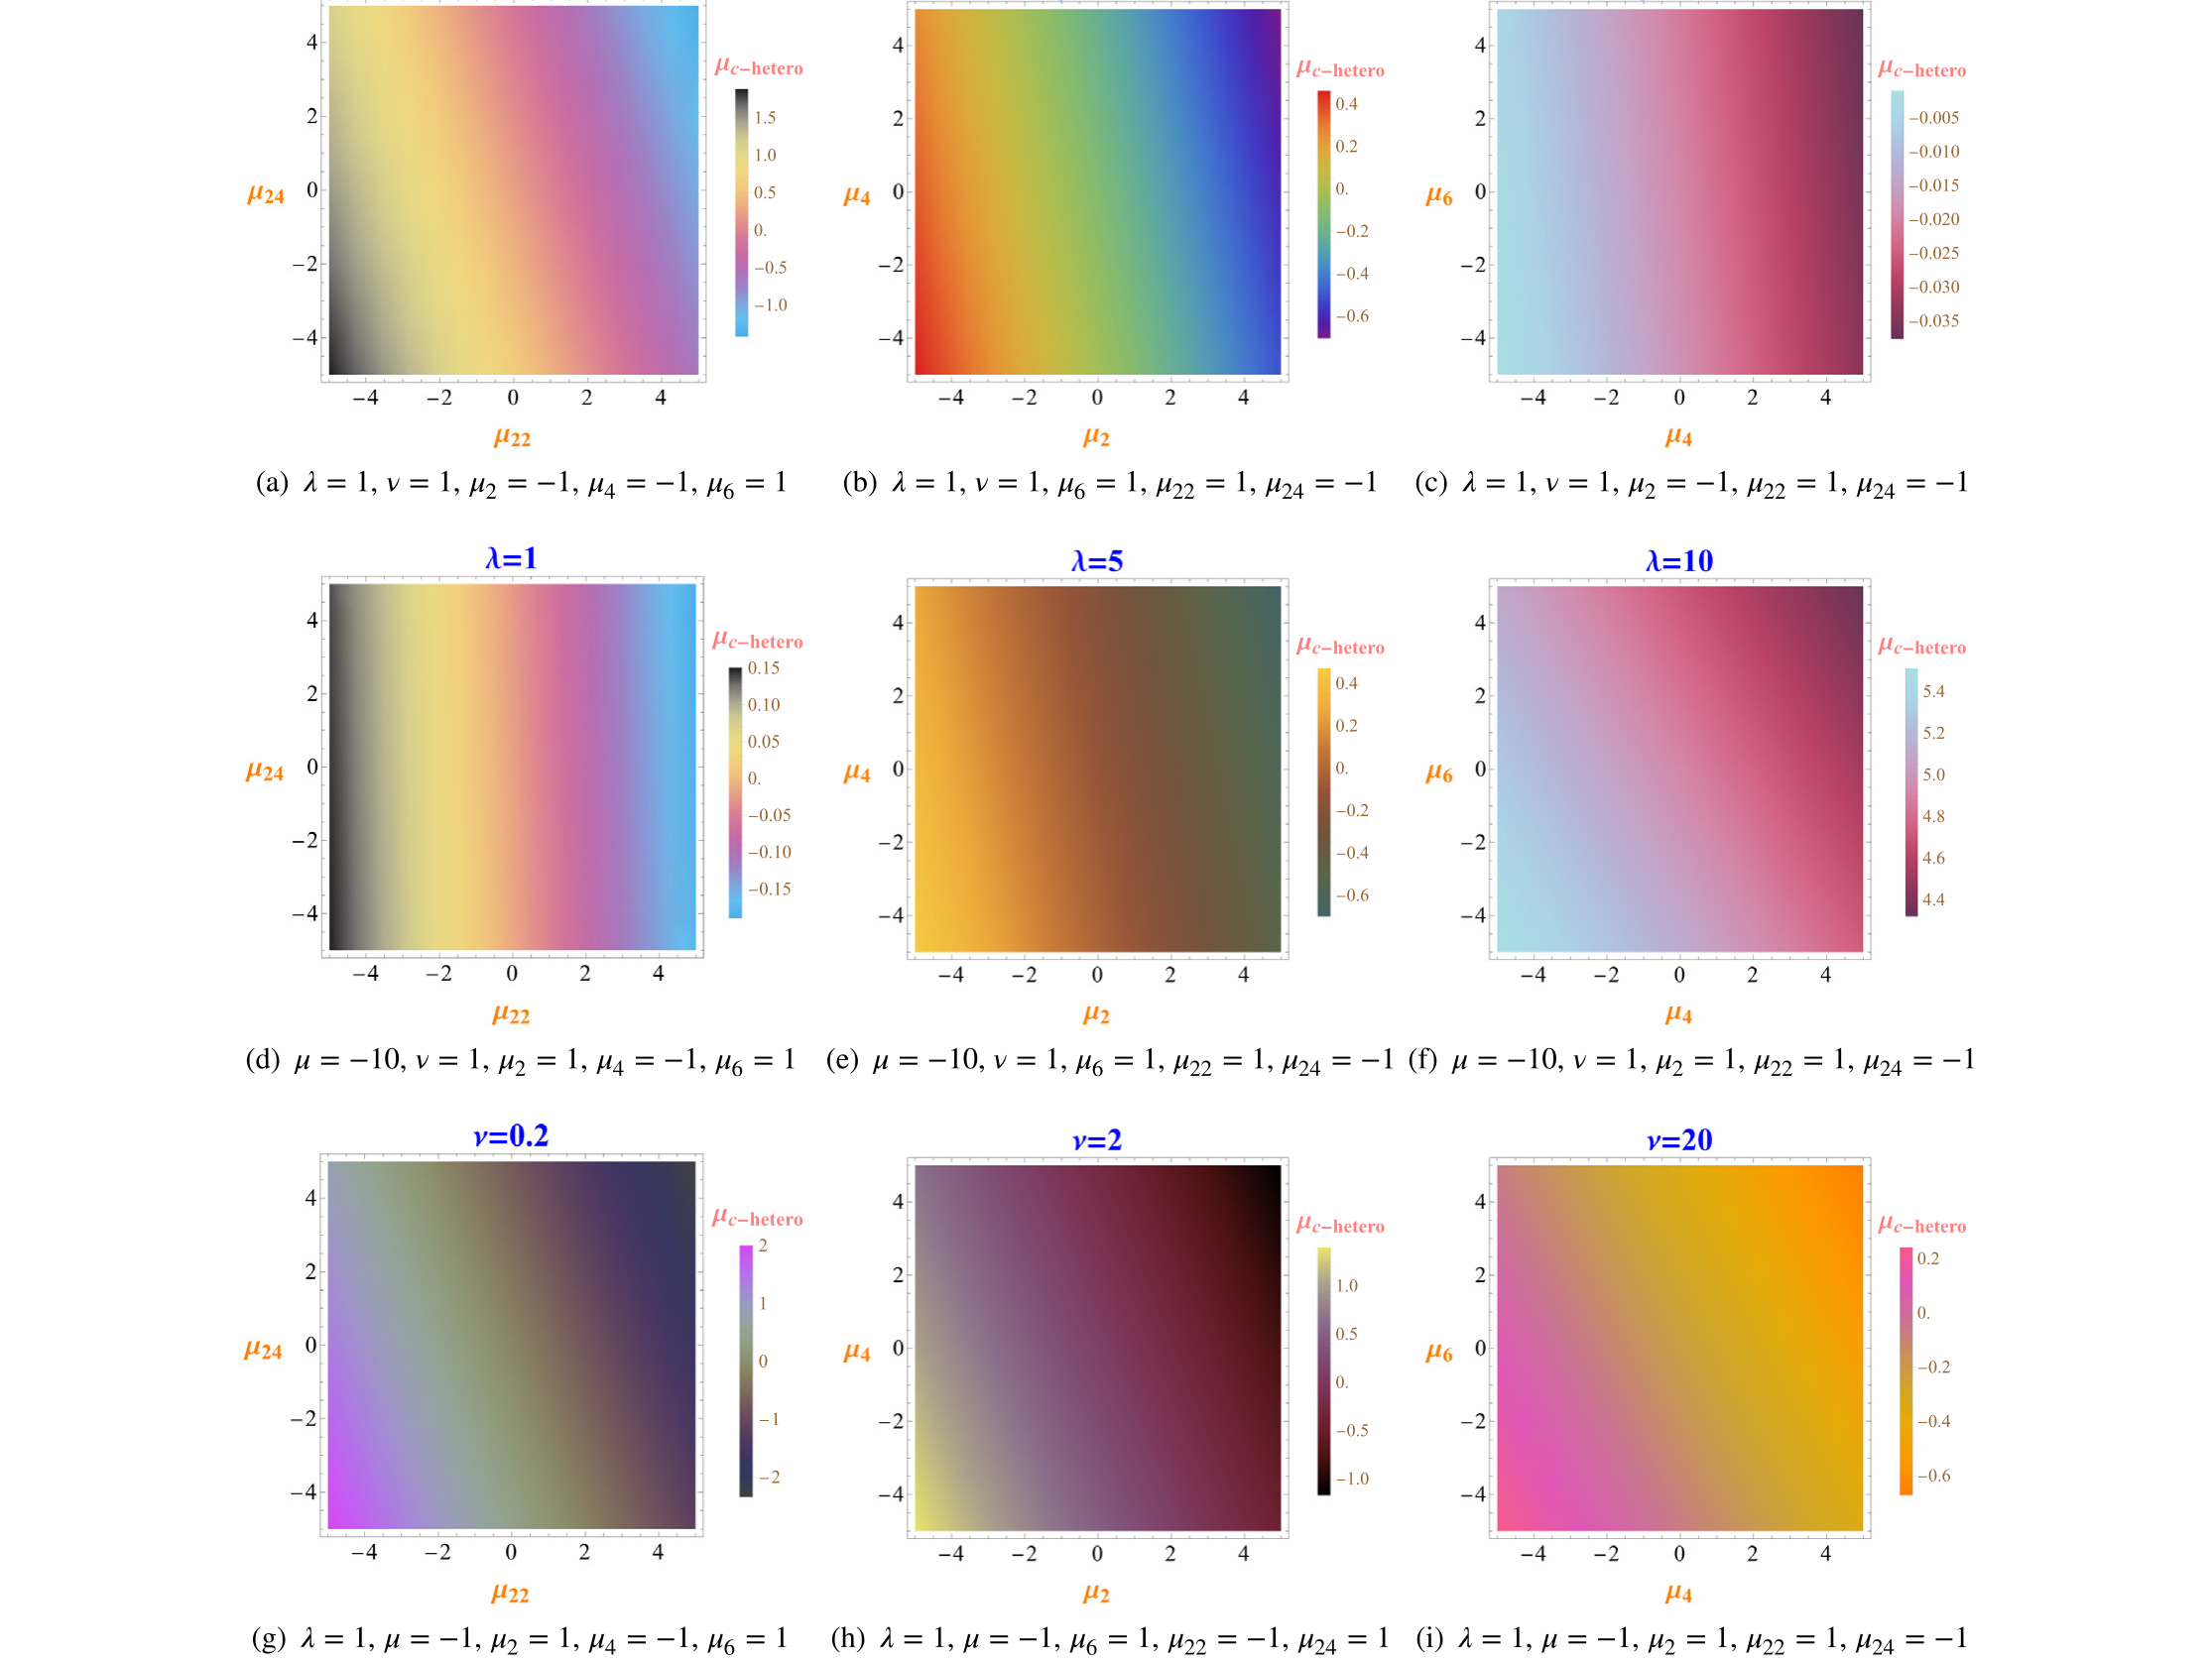
\includegraphics[width=0.85\textwidth]{p3-fig8.png}\\
\captionof{figure}{\textbf{Figure 8.} Variation of the heteroclinic bifurcation parameter $\mu_c^{\mathrm{hetero}}$ with system parameters in different conditions. Each subfigure shows how $\mu_c^{\mathrm{hetero}}$ changes as one damping coefficient is varied while others are fixed.}
\label{fig:fig8}
\end{center}

\begin{center}
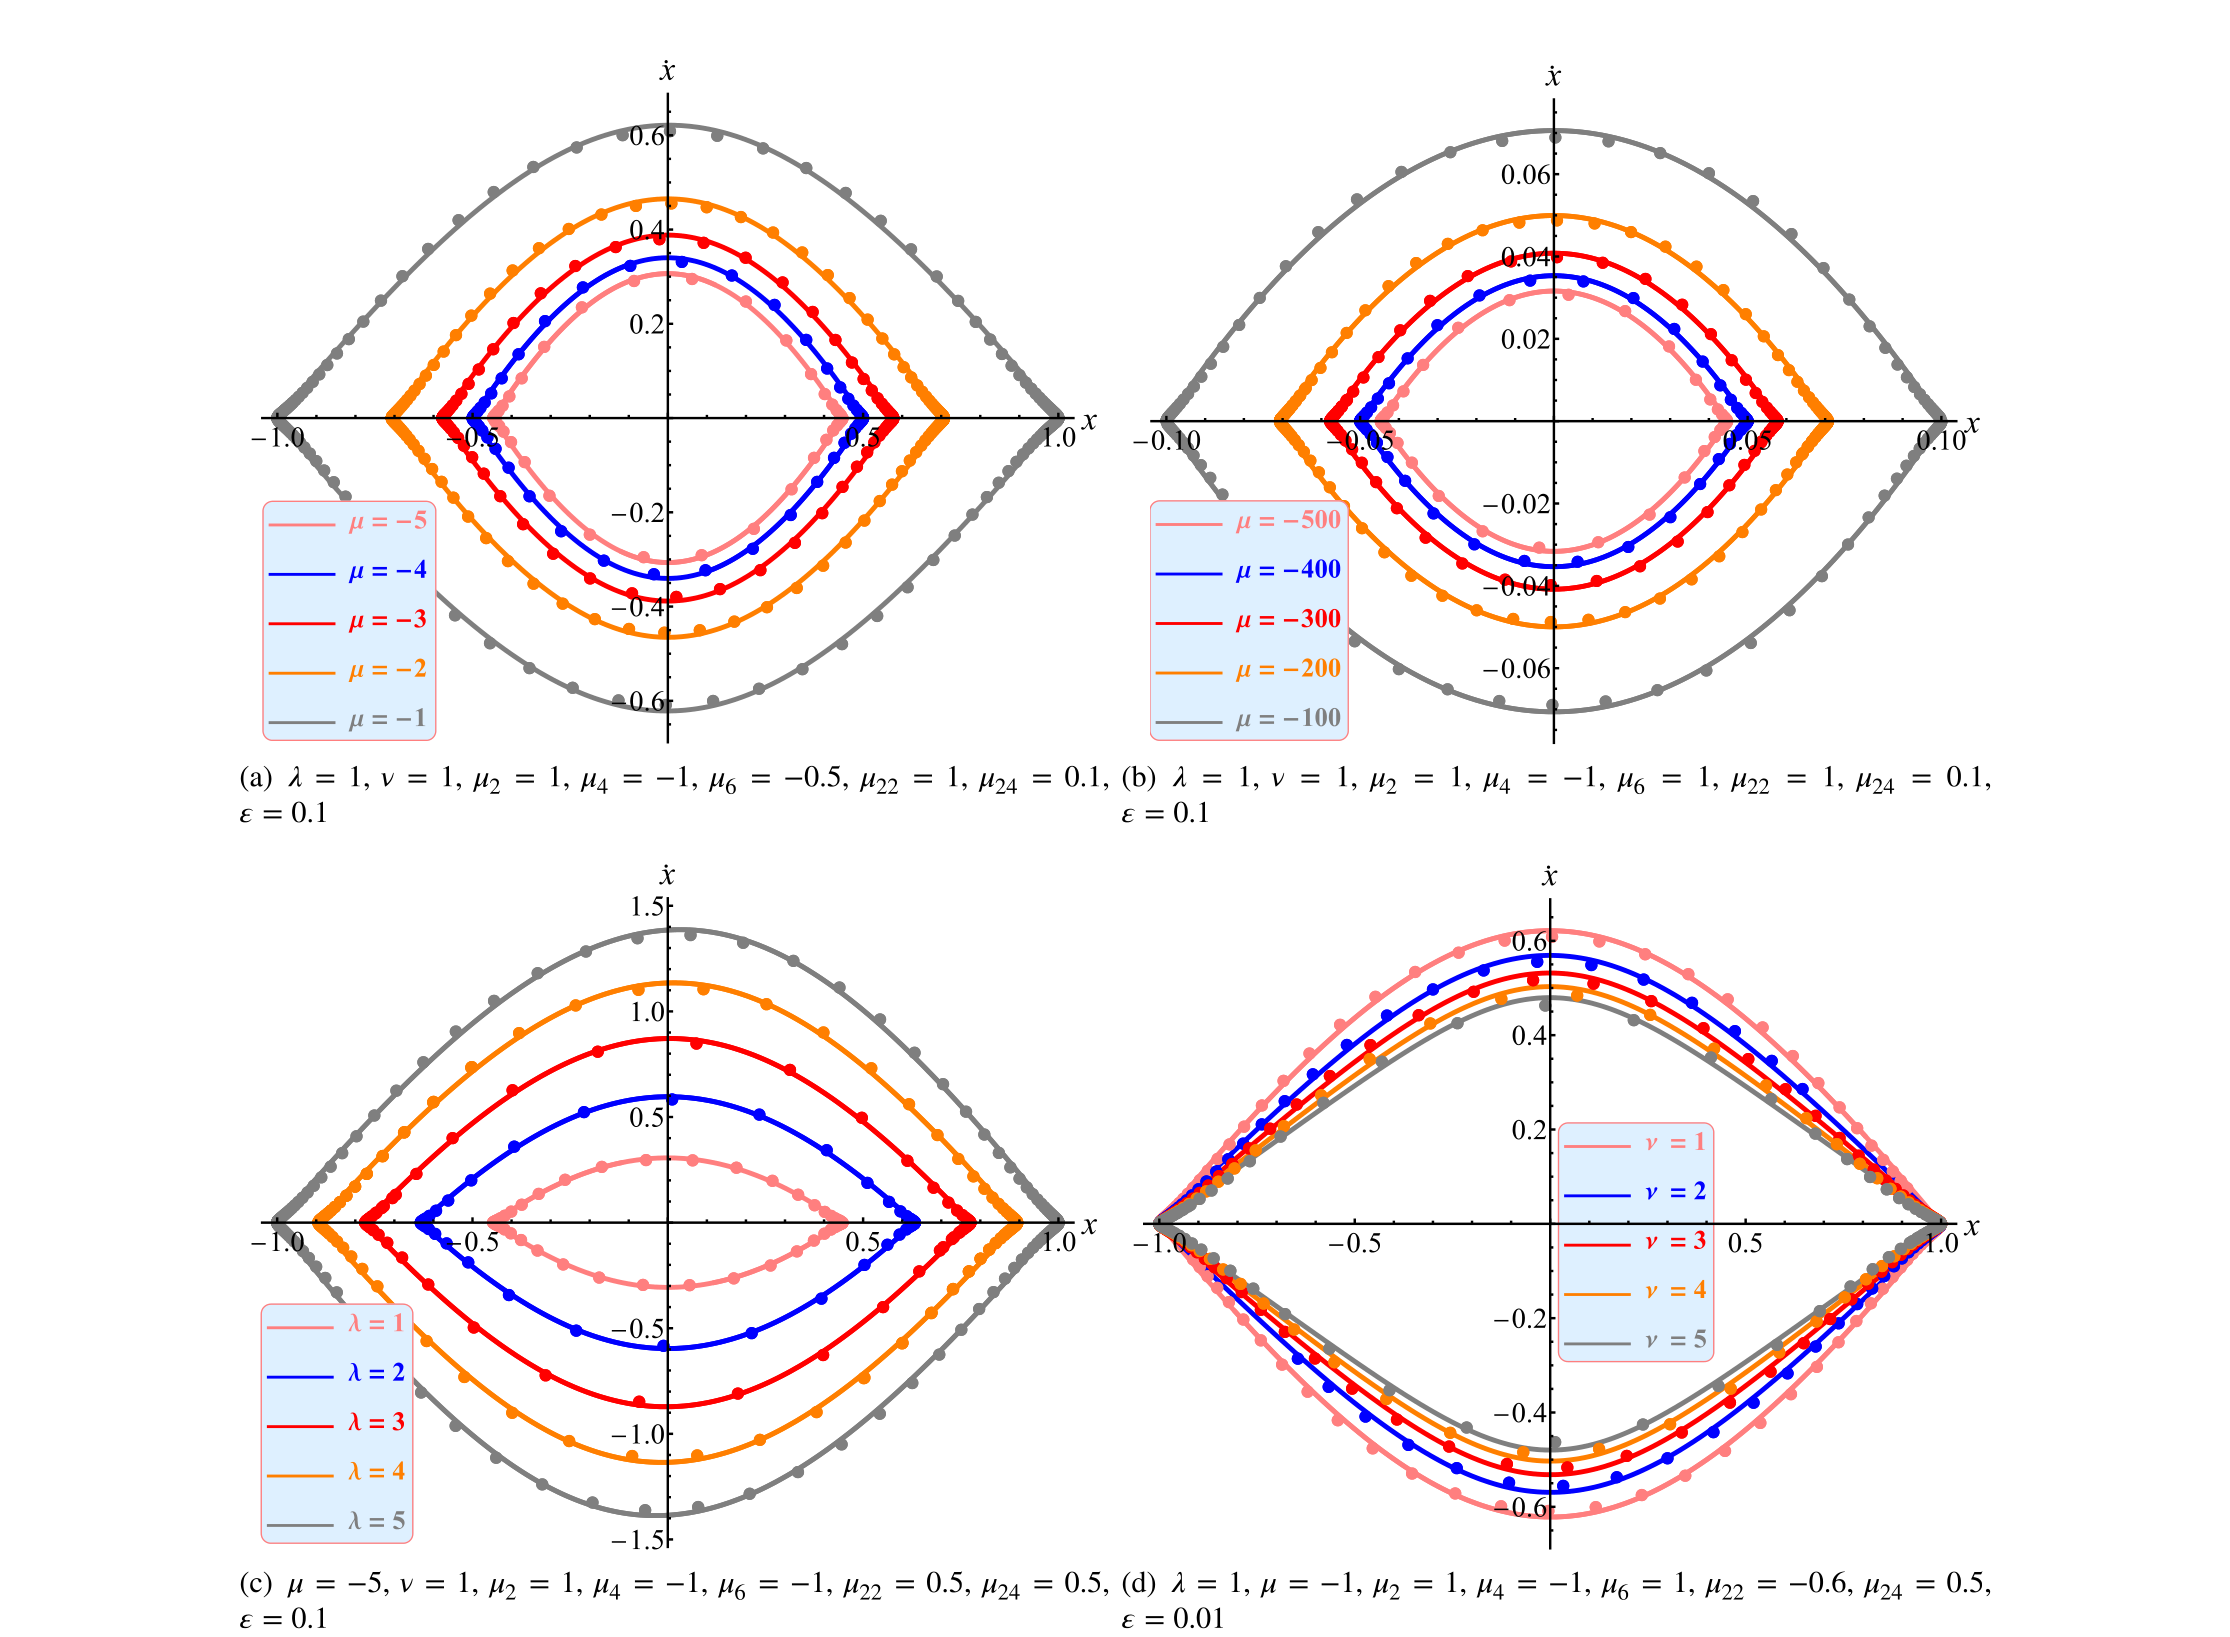
\includegraphics[width=0.85\textwidth]{p3-fig9.png}\\
\captionof{figure}{\textbf{Figure 9.} Phase portraits of heteroclinic solutions with different parameters. Each subfigure compares the analytical MGHFP solution with the Runge--Kutta numerical reference, validating the method's accuracy for heteroclinic orbit prediction.}
\label{fig:fig9}
\end{center}

\section{Key Findings}

\begin{enumerate}[leftmargin=2em]
\item \textbf{First purely symbolic GHFP variant:} The introduction of composite Simpson quadrature into the GHFP framework makes the proposed method the first variant capable of \textbf{purely symbolic execution} for complicated oscillators --- no parameter pre-assignment needed. This is the foundational innovation enabling all subsequent MGHFP work.

\item \textbf{Complete lifecycle from parametric plane (Figures 2--3):} The $\mu_c$--$A$ curve reveals the entire lifecycle of each limit cycle, with four distinct regions separated by semi-stable bifurcation points. Phase portraits in each region visually confirm the parametric analysis.

\item \textbf{Homoclinic and heteroclinic bifurcations predicted (Figures 8--9):} Both types of global bifurcation are quantitatively analyzed. The analytical expression for $\mu_c^{\mathrm{hetero}}$ enables systematic study of its dependence on all damping coefficients simultaneously.

\item \textbf{Method validated on maximally challenging test case:} The DHRL oscillator combines rational restoring force $\frac{\lambda x + \mu x^3}{1+\nu x^2}$ with six-term generalized Rayleigh--Li\'enard damping. All analytical predictions agree with Runge--Kutta results.

\item \textbf{Foundation for the MGHFP series:} This paper establishes the framework subsequently extended to SD oscillators with quartic damping (IJNLM 2025, with Pad\'e enhancement) and coupled SD oscillators with two irrational terms (Phys.\ Scr.\ 2026).
\end{enumerate}

\section{Engineering Significance}

The generalized DHRL oscillator models realistic scenarios in MEMS resonators (squeeze-film damping), vibration isolators (nonlinear electromagnetic damping), and energy harvesting (self-excited systems). The MGHFP method provides the first analytical tool capable of producing continuous amplitude--parameter curves for such systems.

\vfill
\begin{center}
\small\rule{0.5\textwidth}{0.3pt}\\[4pt]
\small\color{primary} Author: Zhenbo Li (lizhenbo@usc.edu.cn)\\
\small ORCID: 0000-0003-2290-971X\\
\small University of South China, School of Mathematics and Physics\\
\small Hunan Key Laboratory of Mathematical Modeling and Scientific Computing
\end{center}

\end{document}
